%% (Master) Thesis template
% Template version used: v1.4
%
% Largely adapted from Adrian Nievergelt's template for the ADPS
% (lecture notes) project.


%% We use the memoir class because it offers a many easy to use features.
\documentclass[11pt,a4paper,titlepage]{memoir}

%% Packages
%% ========

\usepackage{style}

%% LaTeX Font encoding -- DO NOT CHANGE
\usepackage[OT1]{fontenc}

%% Babel provides support for languages.  'english' uses British
%% English hyphenation and text snippets like "Figure" and
%% "Theorem". Use the option 'ngerman' if your document is in German.
%% Use 'american' for American English.  Note that if you change this,
%% the next LaTeX run may show spurious errors.  Simply run it again.
%% If they persist, remove the .aux file and try again.
\usepackage[english]{babel}

%% Input encoding 'utf8'. In some cases you might need 'utf8x' for
%% extra symbols. Not all editors, especially on Windows, are UTF-8
%% capable, so you may want to use 'latin1' instead.
\usepackage[utf8]{inputenc}

%% This changes default fonts for both text and math mode to use Herman Zapfs
%% excellent Palatino font.  Do not change this.
\usepackage[sc]{mathpazo}

%% The AMS-LaTeX extensions for mathematical typesetting.  Do not
%% remove.
\usepackage{amsmath,amssymb,amsfonts,mathrsfs}

%% NTheorem is a reimplementation of the AMS Theorem package. This
%% will allow us to typeset theorems like examples, proofs and
%% similar.  Do not remove.
%% NOTE: Must be loaded AFTER amsmath, or the \qed placement will
%% break
%\usepackage[amsmath,thmmarks]{ntheorem}

%% LaTeX' own graphics handling
\usepackage{graphicx}

%% We unfortunately need this for the Rules chapter.  Remove it
%% afterwards; or at least NEVER use its underlining features.
\usepackage{soul}

%% This allows you to add .pdf files. It is used to add the
%% declaration of originality.
\usepackage{pdfpages}

%% Some more packages that you may want to use.  Have a look at the
%% file, and consult the package docs for each.
%% See the TeXed file for more explanations

%% [OPT] Multi-rowed cells in tabulars
%\usepackage{multirow}

%% [REC] Intelligent cross reference package. This allows for nice
%% combined references that include the reference and a hint to where
%% to look for it.
\usepackage{varioref}

%% [OPT] Easily changeable quotes with \enquote{Text}
%\usepackage[german=swiss]{csquotes}

%% [REC] Format dates and time depending on locale
\usepackage{datetime}

%% [OPT] Provides a \cancel{} command to stroke through mathematics.
%\usepackage{cancel}

%% [NEED] This allows for additional typesetting tools in mathmode.
%% See its excellent documentation.
\usepackage{mathtools}

%% [ADV] Conditional commands
%\usepackage{ifthen}

%% [OPT] Manual large braces or other delimiters.
%\usepackage{bigdelim, bigstrut}

%% [REC] Alternate vector arrows. Use the command \vv{} to get scaled
%% vector arrows.
%\usepackage[h]{esvect}

%% [NEED] Some extensions to tabulars and array environments.
\usepackage{array}

%% [OPT] Postscript support via pstricks graphics package. Very
%% diverse applications.
%\usepackage{pstricks,pst-all}

%% [?] This seems to allow us to define some additional counters.
%\usepackage{etex}

%% [ADV] XY-Pic to typeset some matrix-style graphics
%\usepackage[all]{xy}

%% [OPT] This is needed to generate an index at the end of the
%% document.
%\usepackage{makeidx}

%% [OPT] Fancy package for source code listings.  The template text
%% needs it for some LaTeX snippets; remove/adapt the \lstset when you
%% remove the template content.
\usepackage{listings}
\lstset{language=TeX,basicstyle={\normalfont\ttfamily}}

%% [REC] Fancy character protrusion.  Must be loaded after all fonts.
\usepackage[activate]{pdfcprot}

%% [REC] Nicer tables.  Read the excellent documentation.
\usepackage{booktabs}


%% Our layout configuration.  DO NOT CHANGE.
%%% Memoir layout setup

%% NOTE: You are strongly advised not to change any of them unless you
%% know what you are doing.  These settings strongly interact in the
%% final look of the document.

% Dependencies
\usepackage{ETHlogo}

% Turn extra space before chapter headings off.
\setlength{\beforechapskip}{0pt}

\nonzeroparskip
\parindent=0pt
\defaultlists

% Chapter style redefinition
\makeatletter

\if@twoside
  \pagestyle{Ruled}
  \copypagestyle{chapter}{Ruled}
\else
  \pagestyle{ruled}
  \copypagestyle{chapter}{ruled}
\fi
\makeoddhead{chapter}{}{}{}
\makeevenhead{chapter}{}{}{}
\makeheadrule{chapter}{\textwidth}{0pt}
\copypagestyle{abstract}{empty}

\makechapterstyle{bianchimod}{%
  \chapterstyle{default}
  \renewcommand*{\chapnamefont}{\normalfont\Large\sffamily}
  \renewcommand*{\chapnumfont}{\normalfont\Large\sffamily}
  \renewcommand*{\printchaptername}{%
    \chapnamefont\centering\@chapapp}
  \renewcommand*{\printchapternum}{\chapnumfont {\thechapter}}
  \renewcommand*{\chaptitlefont}{\normalfont\huge\sffamily}
  \renewcommand*{\printchaptertitle}[1]{%
    \hrule\vskip\onelineskip \centering \chaptitlefont\textbf{\vphantom{gyM}##1}\par}
  \renewcommand*{\afterchaptertitle}{\vskip\onelineskip \hrule\vskip
    \afterchapskip}
  \renewcommand*{\printchapternonum}{%
    \vphantom{\chapnumfont {9}}\afterchapternum}}

% Use the newly defined style
\chapterstyle{bianchimod}

\setsecheadstyle{\Large\bfseries\sffamily}
\setsubsecheadstyle{\large\bfseries\sffamily}
\setsubsubsecheadstyle{\bfseries\sffamily}
\setparaheadstyle{\normalsize\bfseries\sffamily}
\setsubparaheadstyle{\normalsize\itshape\sffamily}
\setsubparaindent{0pt}

% Set captions to a more separated style for clearness
\captionnamefont{\sffamily\bfseries\footnotesize}
\captiontitlefont{\sffamily\footnotesize}
\setlength{\intextsep}{16pt}
\setlength{\belowcaptionskip}{1pt}

% Set section and TOC numbering depth to subsection
\setsecnumdepth{subsection}
\settocdepth{subsection}

%% Titlepage adjustments
\pretitle{\vspace{0pt plus 0.7fill}\begin{center}\HUGE\sffamily\bfseries}
\posttitle{\end{center}\par}
\preauthor{\par\begin{center}\let\and\\\Large\sffamily}
\postauthor{\end{center}}
\predate{\par\begin{center}\Large\sffamily}
\postdate{\end{center}}

\def\@advisors{}
\newcommand{\advisors}[1]{\def\@advisors{#1}}
\def\@department{}
\newcommand{\department}[1]{\def\@department{#1}}
\def\@thesistype{}
\newcommand{\thesistype}[1]{\def\@thesistype{#1}}

\renewcommand{\maketitlehooka}{\noindent\ETHlogo[2in]}

\renewcommand{\maketitlehookb}{\vspace{1in}%
  \par\begin{center}\Large\sffamily\@thesistype\end{center}}

\renewcommand{\maketitlehookd}{%
  \vfill\par
  \begin{flushright}
    \sffamily
    \@advisors\par
    \@department, ETH Z\"urich
  \end{flushright}
}

\checkandfixthelayout

\setlength{\droptitle}{-48pt}

\makeatother

% This defines how theorems should look. Best leave as is.
\theoremstyle{plain}
\setlength\theorempostskipamount{0pt}

%%% Local Variables:
%%% mode: latex
%%% TeX-master: "thesis"
%%% End:


%% Theorem environments.  You will have to adapt this for a German
%% thesis.
%%% Theorem-like environments

%% This can be changed according to language. You can comment out the ones you
%% don't need.

\numberwithin{equation}{chapter}

%% German theorems
%\newtheorem{satz}{Satz}[chapter]
%\newtheorem{beispiel}[satz]{Beispiel}
%\newtheorem{bemerkung}[satz]{Bemerkung}
%\newtheorem{korrolar}[satz]{Korrolar}
%\newtheorem{definition}[satz]{Definition}
%\newtheorem{lemma}[satz]{Lemma}
%\newtheorem{proposition}[satz]{Proposition}

%% English variants
\newtheorem{theorem}{Theorem}[chapter]
\newtheorem{example}[theorem]{Example}
\newtheorem{remark}[theorem]{Remark}
\newtheorem{corollary}[theorem]{Corollary}
\newtheorem{definition}[theorem]{Definition}
\newtheorem{lemma}[theorem]{Lemma}
\newtheorem{proposition}[theorem]{Proposition}

%% Proof environment with a small square as a "qed" symbol
\theoremstyle{nonumberplain}
\theorembodyfont{\normalfont}
\theoremsymbol{\ensuremath{\square}}
\newtheorem{proof}{Proof}
%\newtheorem{beweis}{Beweis}


%% Helpful macros.
%%% Custom commands
%% ===============

%% Special characters for number sets, e.g. real or complex numbers.
\newcommand{\C}{\mathbb{C}}
\newcommand{\K}{\mathbb{K}}
\newcommand{\N}{\mathbb{N}}
\newcommand{\Q}{\mathbb{Q}}
\newcommand{\R}{\mathbb{R}}
\newcommand{\Z}{\mathbb{Z}}
\newcommand{\X}{\mathbb{X}}

%% Fixed/scaling delimiter examples (see mathtools documentation)
\DeclarePairedDelimiter\abs{\lvert}{\rvert}
\DeclarePairedDelimiter\norm{\lVert}{\rVert}

%% Use the alternative epsilon per default and define the old one as \oldepsilon
\let\oldepsilon\epsilon
\renewcommand{\epsilon}{\ensuremath\varepsilon}

%% Also set the alternate phi as default.
\let\oldphi\phi
\renewcommand{\phi}{\ensuremath{\varphi}}


%% Make document internal hyperlinks wherever possible. (TOC, references)
%% This MUST be loaded after varioref, which is loaded in 'extrapackages'
%% above.  We just load it last to be safe.
\usepackage[linkcolor=black,colorlinks=true,citecolor=black,filecolor=black]{hyperref}


%% Document information
%% ====================

\title{Strong and Secure Access Control in PostgreSQL}
\author{Mohammed Ajil}
\thesistype{Bachelor Thesis}
\advisors{Advisors: Prof.\ Dr.\ D. Basin, M. Guarnieri}
\department{Department of Computer Science}
\date{March 21, 2016}

\begin{document}

\frontmatter

%% Title page is autogenerated from document information above.  DO
%% NOT CHANGE.
\begin{titlingpage}
  \calccentering{\unitlength}
  \begin{adjustwidth*}{\unitlength-24pt}{-\unitlength-24pt}
    \maketitle
  \end{adjustwidth*}
\end{titlingpage}

%% The abstract of your thesis.  Edit the file as needed.
\begin{abstract}
  This example thesis briefly shows the main features of our thesis
  style, and how to use it for your purposes.
\end{abstract}


%% TOC with the proper setup, do not change.
\cleartorecto
\tableofcontents
\mainmatter

%% Your real content!
\section{Introduction}
To protect the confidentiality of sensitive information stored in databases, it is essential to restrict access to the data.
%
For this, the SQL standard defines an access control model, and existing Database Management Systems (DBMSs) have accordingly implemented it. 
%
One of the main tasks of database access control mechanisms is to check whether \texttt{SELECT} queries issued by the users are secure.
%
This is \emph{essential} to effectively secure database systems and prevent the leakage of sensitive information.

The access control mechanism implemented in PostgreSQL is rather simple.
%
It just analyzes the syntax of submitted \texttt{SELECT} queries.
%
Namely, a \texttt{SELECT} query is deemed secure if all the tables and views referenced in it are readable to the user issuing the query, according to the access control policy.
%
This mechanism is overly restrictive.
%
Indeed, as already identified in~\cite{...}, even queries not satisfying this criterion are secure.

Recently, Guarnieri et al.~\cite{guarnieri2016strong} investigated the limitations of this access control model. 
%
They developed a novel, more secure, access control mechanism.
%
This access control mechanism shows that sub-routines for checking the security of \texttt{SELECT} queries are also one of the main building blocks of strong access control mechanisms such as the one proposed.
%
The mechanism however also requires that these routines are more permissive and efficient, to keep the overall database system still usable.
%
Motivated by this Guarnieri et al. developed such a routine for checking the security of \texttt{SELECT} statements.

The routine proposed in~\cite{guarnieri2016strong} however, has two main practical limitations.
%
First, it is based on the relational calculus, whereas existing DBMSs are based on SQL. Despite SQL being inspired by the relational calculus it differs from it in significant ways. For instance, they differ in their syntax and semantics, e.g., SQL uses a bag semantics whereas the relational calculus relies on a set-based semantics.
%
Second, it is defined primarily for boolean queries, whereas \texttt{SELECT} queries usually retrieve tuples.
%
Even though boolean queries can be used to encode the result of non-boolean queries, this encoding may introduce a extreme blow-up in the formula's size.

Motivated by the idea of extending the mechanism from~\cite{guarnieri2016strong} to the entire SQL language, in this thesis we develop a novel algorithm for checking the security of \texttt{SELECT} queries.
%
Our algorithm extends the one proposed by Guarnieri et al. to the SQL language and is more permissive than the one implemented in PostgreSQL.

\smallskip
\noindent
{\bf Contributions.}
%
Due to the gravity of the current situation, where the mentioned attacks can cause severe damage, this thesis explores the possibility of preventing confidentiality attacks in PostgreSQL, a widely used DBMS.
%
First, we refactor the original PostgreSQL's implementation to isolate the access control mechanism and provide a general interface for access requests, independent of the type of query.
%
The original implementation requires a deep understanding of the backend architecture of PostgreSQL to be able to extend and improve the current access control algorithm.
%
Our refactoring provides the possibility of improving and extending access control without interfering with the internals of the DBMS.

Second, we extend the access control mechanism proposed by Guarnieri et al.~\cite{guarnieri2016strong} to SQL.
%
This is essential to effectively secure PostgreSQL and prevent leakages of sensitive information.
%
In more detail, we implemented a new access control mechanism for \texttt{SELECT} queries, which, as mentioned before, represents the first building block of successfully implementing the access control mechanism proposed by Guarnieri et al.
%
\remark{
As shown in our experiments, our mechanism introduces an overhead, on average, of XX\%, in contrast to Guarnieri et al.'s mechanism  that  has an overhead of ...X\cite{guarnieri2016strong}.
}

\smallskip
\noindent
{\bf Organization.}
%
In chapter 2 we will introduce some motivating examples.
%
In chapter 3 we will give background information to access control by comparing current access control mechanism to the model introduced in~\cite{guarnieri2016strong}.
%
After that we will introduce the architecture of PostgreSQL and the new access control algorithm in chapter 4. 
%
In chapter 5 we will begin by showing the formal models of all aspects of the new security defintions and how they are extended from the relational algebra to SQL. 
%
Furthermore we will conduct experiments with state-of-the-art benchmark databases and queries in chapter 6. 
%
In chapter 7 we will introduce some related work to the thesis. 
%
Finally in chapter 8 the conclusions are drawn and future possibilities are discussed.
\section{Motivating Examples}

We show here how attackers can exploit advanced features of DBMSs to perform attacks on the system as presented in~\cite{guarnieri2016strong}.
%
These attacks are classified in two families: \emph{Integrity attacks} and \emph{Confidentiality attacks}.
%
In the former, the attacker is able to make unauthorized changes to the database, thus violating the integrity of the database from a security point of view.
%
In the latter, the attacker manages to learn sensitive information from the database, that according to the security policy, should not be disclosed to the attacker.
%
Guarnieri et al. have mounted these attacks manually against several widely used DBMS with shocking results: No existing access control mechanism is able to fully prevent these attacks.

\subsection{Integrity Attacks}

Here we present integrity attacks. 
%
The following attacks use \texttt{INSERT}, \texttt{DELETE}, \texttt{GRANT}, and \texttt{REVOKE} commands together with views and triggers, which are procedures automatically executed by the DBMS in response to user commands.

In the first attack the attacker will use triggers to execute an unauthorized command on the database system. The trigger will be executed by an unaware user with a higher security clearance.

\begin{attack}
\bf{Trigger with activator's privileges:}
Consider a database with two tables $P$ and $S$ and two users $u$ and $w$. The attacker is the user $u$ whose goal is to delete the contents of $S$. The policy is as follows: $u$ is not authorized to alter $S$, $u$ can create triggers on $P$, and $w$ can read and modify $S$ and $P$. The attack is as follows:
\begin{enumerate}
\item $u$ creates the following trigger:
	\begin{verbatim}
	CREATE TRIGGER t ON P AFTER INSERT
    DELETE * FROM S
	\end{verbatim}
\item $u$ waits until $w$ insers a tuple into the table $P$. The trigger will then be invoked using $w$'s and $S$'s content will be deleted.
\end{enumerate}
\end{attack}

By replacing the \texttt{DELETE} command inside the trigger with a \texttt{GRANT} command an attacker can also escalate his privileges.

In the second attack the attacker will use views to escalate his privileges. He will delegate read privileges, without having the necessary permissions on the origin table.

\begin{attack}
\bf{Grating views:}
Consider a database with a table $S$ and two users $u$ and $v$, and the following policy: $u$ can create views and read $S$, but cannot delegate read permissions on $S$. $v$ cannot read $S$. The attacker is $u$ who will allow the unprivileged user $v$ to read the contents of $S$:
\begin{enumerate}
\item $u$ creates the view $V$:
	\begin{verbatim}
	CREATE VIEW V AS
	SELECT * FROM S;
	\end{verbatim}
\item $u$ issues the command:
	\begin{verbatim}
	GRANT SELECT ON V TO v;
	\end{verbatim}
\end{enumerate}
Now $v$ can read the contents of $S$ through $V$.
\end{attack}

\subsection{Confidentiality Attacks}

In the following we will present confidentiality attacks.




\section{Background}

In this section it is shown why the current access control mechanisms are flawed by contrasting the current access control mechanism in PostgreSQL with the new access control mechanism based on~\cite{guarnieri2016strong}.
%
\subsection{Current access control mechanism in PostgreSQL}
%
The access control mechanism used in PostgreSQL is to large extent an implementation of the access control model defined by the SQL standard.
%
This standard makes the assumption that information can only be leaked through \texttt{SELECT} queries issued to the DBMS.
%
The conclusions made in the following paragraphs are backed by an analysis of the backend code of PostgreSQL, since a proper documentation of the internals is missing.

The administrator has to define an access control policy for the database.
%
This policy defines how users can interact with the system.
%
A database object can refer to any structure within a database: tables, views, triggers, functions etc.
%
For each object the administrator has to define \emph{access control lists} (ACLs) for each database role.
%
The administrator can define an ACL for the public, a group or a user. 
%
These ACLs then define the privileges to a database object for a database role.
%
The privileges among others include creation of tables, views or triggers in the database or reading, altering or deleting of tuples from tables or views.
%
These privileges can be modified using \texttt{GRANT} or \texttt{REVOKE} commands, whereas the execution of those is also based on the ACLs.
%
The possible privileges include insert, update, select, create, execute etc.\footnote{\url{http://www.postgresql.org/docs/9.5/static/sql-grant.html}}
%
Depending on the object different privileges are applicable. For example the execution privilege is only applicable to functions and triggers, whereas the insert privilege is only applicable to tables or views.
%
When issuing a query to the database, depending on the query, a function is executed which, among other things, retrieves the ACL for the objects referenced in the query and checks if the required privileges are available for the user issuing the command.
%
When deciding if a \texttt{SELECT} query is authorized, we can distinguish two cases: 
%
In the first case the user issuing the query has read privileges on all the relations in the \texttt{FROM} clause of the query, then security is trivial and we can allow the query. 
%
In the second case the user does not have read privileges on all the tables in the \texttt{FROM} clause of the query. 
%
The current access control mechanism will not authorize this query.
%
The access control mechanism implemented in PostgreSQL does not take into account other aspects of the database system, i.e., in the case of an \texttt{INSERT} query there is no check if the execution of triggers might reveal information to an attacker.
%
The attacks in the previous section succeed because of this behaviour.
%
\remark{What should I add here? I could explain the process that happens for a \texttt{SELECT} in detail here, it will sound complicated but boil down to comparing bits in the ACL, what do you think?}
%
\subsection{New access control mechanism}
%
The approach taken in the access control mechanism based on the model proposed in~\cite{guarnieri2016strong} is different.
%
The basis for creating an access control policy are still ACLs, but the basis for deciding if a command is allowed to be executed is the resulting behaviour of the database system.

\remark{Can we talk about how to continue here? I think this is a bit unclear to me and to the reader. As you mentioned we need a good example here that can explain the situation}
\section{Architecture}


Here, we introduce the architecture of the current version of PostgreSQL.
%
We also show how the architecture looks after the refactoring and implementation of the new algorithm.
%
\subsection{Current architecture}
%
In the current version of PostgreSQL the access control module is not identifiable as a stand-alone module in the backend code of the DBMS.
%
Figure~\ref{figure:postgresql:architecture} shows a flowchart of a PostgreSQL server instance.
%
The flowchart shows backend's behaviour.
%
\subsubsection{Backend architecture}
%
Each box in the flowchart represents a module of PostgreSQL.

The \emph{Main} module is responsible for checking the underlying system requirements, such as the system user starting the server, available memory etc. If all the requirements are met the {Postmaster} process is started.

The \emph{Postmaster} is the starting point for any PostgreSQL server instance. 
%
In this module, system setup tasks such as loading the data representing the database and setting up listeners for database connections are executed.
%
After setting everything up, the Postmaster waits for a connection request from a \emph{frontend application}, i.e., any application that connects to the database.
%
When receiving a connection request, the Postmaster forks itself.
%
The child process then will either authorize the request and become a \emph{Backend} or reject the request and exit.
%
All the blue boxes in the flowchart represent modules of the Backend of a PostgreSQL server.

The Backend consists of an infinite loop that breaks at the parser stage.
%
At this point the Backend is ready to receive a query from the connected frontend application.
%
After receiving a query in text form, the parser creates the abstract syntax tree representing the query.
%
The abstract syntax tree is then passed to the \emph{Traffic Cop}.

The Traffic Cop first analyzes the query to classify it either as a {utility query} or {non-utility query}.
%
\emph{Utility queries} modify the structure of the database, e.g., they create or drop a table, view, or  trigger.
%
\emph{Non-utility queries}, instead, act on the data inside the database.
%
For instance, \texttt{SELECT}, \texttt{DELETE}, and \texttt{UPDATE} are all non-utility queries. 
%
After determining the type, the Traffic Cop forwards utility queries to the \emph{Utility Command} module, which checks the authorization of the query and, if the query is authorized, executes it.

Non-utility commands are forwarded to the \emph{Rewrite Query} module.
%
Here the query is rewritten according to the \emph{PostgreSQL Rule System}.
%
The PostgreSQL Rule System is a collection of rules on how to rewrite queries in such a way that the other modules of the Backend can optimize the query as good as possible.
The Rule System, for instance, expands views to their respective definition, allowing the Generate Paths module to produce more comprehensive execution paths.
%
After the rewriting, the rewritten query is passed to the \emph{Generate Paths} module.
%
Here the system generates different \emph{paths} to execute the query.
%
Each path represents a way of executing the query, i.e., a possible way of traversing the abstract syntax tree.
%
According to internal rules the system will choose the optimal path.
%
This path is passed to the \emph{Generate Plan} module, which internally will generate a \emph{plan} for the executor.
%
A plan is detailed guide for the executor on how to retrieve the tuples.

This plan is then forwarded to the executor, which will execute it and return the tuples to the frontend application.
%
\begin{figure}[!ht]
  \centering
    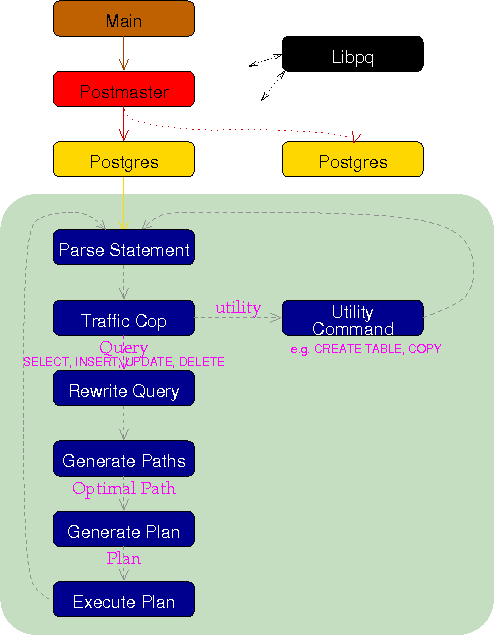
\includegraphics[width=1\textwidth]{img/backend_flowchart.png}
    \caption{Backend Flowchart PostgreSQL \protect \footnotemark}\label{figure:postgresql:architecture}
\end{figure}
%
\footnotetext{\url{http://www.postgresql.org/developer/backend}}
\subsubsection{Access Control}
%
Access control decisions can be made in any of the the following modules: Traffic cop, Executor, or in the module that handles the utility queries.
%
The functions making these decisions, however, also prepare the system for the upcoming change, by, for instance, returning the address where a new table is allocated.
%
Due to the distribution and inconsistency of the access control mechanism, there is no uniform interface that can be called for such a decision.
%
Furthermore,  the mechanism is, sometimes, closely connected to the internals of the database, making the implementation of a new mechanism nearly impossible without refactoring the code.
%
For instance, checking the authorization of \texttt{SELECT} queries is done very late, namely in the executor.
%
This check is on an internal datastructure that represents the tables referenced in the query.
%
Therefore, we need to modify the behaviour of the executor just to modify the way \texttt{SELECT} queries are authorized.
\remark{Very good! This is the kind of information we need to motivate the refactoring :-) We can even use a light version of this to strengthen  the contributions.}
%
\remark{Add some glue, such as ``This is what motivated us to refactor PostgreSQL blah blah...''}

%
\FloatBarrier

%
\subsection{Refactoring}
%
After analyzing the backend, by executing each type of query and following the backend through the process with a debugger, all the functions or code regions relevant to making access control decisions were identified.
%
This identification allowed us to gradually move the code to an external module and build a uniform interface, which is called inside the Traffic cop, when the backend expects a decision. \remark{decision on what?} 

The building of a uniform interface introduced several engineering challenges. \remark{I wouldn't call them challenges. They are design choices (or decisions)}
%
The first decision was to create a stand-alone module in the backend of PostgreSQL dedicated to access control.
This allows developers to clearly identify the code that is responsible for authorizing any type of query.
%
Second we built an interface, that can be called from any module, when requiring an access control decision.

The interface looks as follows:
%
\begin{lstlisting}[frame=single, style=customc]
ac_return_data authorized(ac_decision_data *decision_data);
\end{lstlisting}
%
The structs used in the interface are extensible. For each type of query there is a field in both structs, which represent the input and output data for the all queries of this type.
%
The structs look as follows: \remark{The structs should be explained a bit more. The comments in the code do not give too much information. For instance, why do you have all this stuff? Where do they come from?}
\begin{lstlisting}[frame=single, style=customc]
union ac_return_data_struct {
	/* Returned if CREATE is authorized otherwise NULL*/
	Oid target_namespace; 
	/* Returned if GRANT is authorized otherwise NULL*/
	AclMode current_privileges; 
	/* Returned for Non-utility query */
	bool execute; 
};

struct ac_decision_data_struct {
	/* Tag identifying query */
	command_type command;
	/* If (command == CREATE_RELATION) this cannot be NULL */
	ac_create_relation_data *create_relation_data; 
	/* If (command == GRANT || command == REVOKE) this cannot be NULL */
	ac_grant_data *grant_data; 
	/* If (command == INSERT || command == DELETE || command == SELECT) this cannot be NULL */
	ac_nutility_data *nutility_data; 
	/* If (command == CREATE_TRIGGER) this cannot be NULL */
	ac_create_trigger_data *create_trigger_data; 
};
\end{lstlisting}
%
Each field in the decision data struct is actually a pointer that refers to a struct, which in turn holds all information needed for deciding if the respective type of query is authorized.
%
For instance, the struct that is required to check the authorization of \texttt{GRANT} or \texttt{REVOKE} queries looks as follows:
%
\begin{lstlisting}[frame=single, style=customc]
/* Data needed for deciding on GRANT queries */
struct ac_grant_data_struct {
	bool is_grant;
	AclMode avail_goptions;
	bool all_privs;
	AclMode privileges;
	Oid objectId;
	Oid grantorId;
	AclObjectKind objkind;
	const char *objname;
	AttrNumber att_number;
	const char *colname;
};
\end{lstlisting}
%
This structure actually represents the argument list of the original function that authorizes \texttt{REVOKE} and \texttt{GRANT} queries.
%
Any function that calls this interface will pass all the data needed to make the decision.
%
Depending on the data received, the interface internally calls the functions that were previously distributed among the modules.
%
This allows future developers to gradually implement a new algorithm, by identifying the query received, and either return the result of a new algorithm, or call the original function responsible for the query.
%
To facilitate the identification of the received query,  we have included an additional field in the decision data, which tells exactly what type of query was received by the interface, e.g., \texttt{INSERT} or \texttt{UPDATE} instead of just identifying it as a non-utility query.

We also added a stack that, at any point of the execution of the database system, holds all queries that are not yet completed. \remark{Unclear what complete means}
%
This allows developers to always have a clear view on the state of the database system.
%
The top element of the stack represents the currently executing query.
%
Elements are popped from the stack after the database transaction is completed. \remark{??? which transaction. This comes out of the blue.}
% 
\remark{What about concurrency?}
Each stack's element is a struct that looks as follows:
%
\begin{lstlisting}[frame=single, style=customc]
/* Data structure representing context */
struct ac_context_struct{
	Oid user;
	Oid invoker;
	Query *query;
	const char *query_string;
	bool authorized;
	bool rewritten;
	bool authorizesnext;
};
\end{lstlisting}
%
Each context contains the session user that is connected to the database and the \emph{invoker} of the query.
%
The invoker is relevant if the query is executed under other privileges than the ones of the session user, this happens for instance when a trigger is executed under \emph{owner's privileges}, which means under the privileges of the user that created the trigger.
%
A context also contains the query in text form and as a parsed abstract syntax tree.
%
Also we included three boolean values: ``authorized'' indicates if the query is authorized, ``rewritten'' tells us if the query was rewritten as part of the access control mechanism, and ``authorizesnext'' is used if the query authorizes the query that is below in the context stack. 
\remark{Explain why we need those.}
%
The stack is used to simplify the implementation of novel mechanisms such as the one in~\cite{guarnieri2016strong}, since the algorithm from Guarnieri et. al requires knowledge about other aspects of the system such as triggers being executed, or nested queries.
%
After the process of refactoring it is possible to integrate any access control mechanism as a plug-in.

\appendix

\section{Appendix}

\backmatter

\bibliographystyle{plain}
\bibliography{refs}

\includepdf[pages={-}]{declaration-originality.pdf}

\end{document}
